\documentclass[12pt,a4paper]{article}

%format papier et marges
\usepackage{geometry}
\geometry{
 a4paper,
 total={150mm,227mm},
 left=30mm,
 top=30mm,
 }

\usepackage{styles}

\title{Physique des dispositifs électroniques et des lignes de transmission (LELEC1755)}
\author{\textit{Réalisé par}\\ \textbf{Quentin Aubecq}\\\textit{avec l'aide de}\\ \_ \\\textit{relu par}\\ \_}
\date{2026}

\begin{document} 

\subfile{couverture}

\renewcommand*\contentsname{Table des matières}
\tableofcontents

\break

\section{Équations de Maxwell}

\subsection{Champ électromagnétique : Rappels}

\subsubsection{Loi de Coulomb}

Des charges électriques immobiles créent un champ électrique

\begin{align*}
\vec{E} &= \frac{q}{4\pi\epsilon_0 r^2} \hat{r} \\
        &= \frac{1}{4\pi\epsilon_0} \int_{V'} \frac{(\vec{r} - \vec{r'})}{|\vec{r} - \vec{r'}|} \frac{\rho dv'}{|\vec{r} - \vec{r'}|^2}
\end{align*}

Ce champ est conservatif et dérive d'un potentiel

\subsubsection{Lois de Biot-Savart et Ampère}

Des courants constants (charges en MU) créent un champ magnétique constant

\begin{align*}
\vec{B} &= \frac{\mu_0}{4\pi} \int \frac{I d\vec{l} \times \hat{r}}{r^2} \\
&= \frac{\mu_0}{4\pi} \int_{V'} \frac{\vec{J}(\vec{r'}) \times (\vec{r} - \vec{r'})}{|\vec{r} - \vec{r'}|^3} dv'
\end{align*}

$$\oint \vec{H} \cdot d\vec{l} = I$$

\subsubsection{Force de Lorentz}

$$\vec{F} = q(\vec{E} + \vec{v} \times \vec{B})$$
$$d\vec{F} = I d\vec{l} \times \vec{B}$$

\subsubsection{Loi de Lenz-Faraday}

Un flux/champ magnétique variable crée un champ électromoteur (emf), même s'il n'y a pas de conducteur

$$\epsilon_{ind} = \oint\limits_{C \text{fermé!}} \vec{E}_{emf} \cdot \vec{dl} = - \frac{d\Phi_B}{dt} \neq 0$$

\subsubsection{Onde électromagnétique}

Un champ magnétique variable crée un champ électrique (Lenz-Faraday)

Un champ électrique variable crée un champ magnétique (courant de déplacement)

Des charges électriques accélérées sont responsables de l'apparition d'une one électromagnétique


\subsection{Équations de Maxwell}

\begin{center} 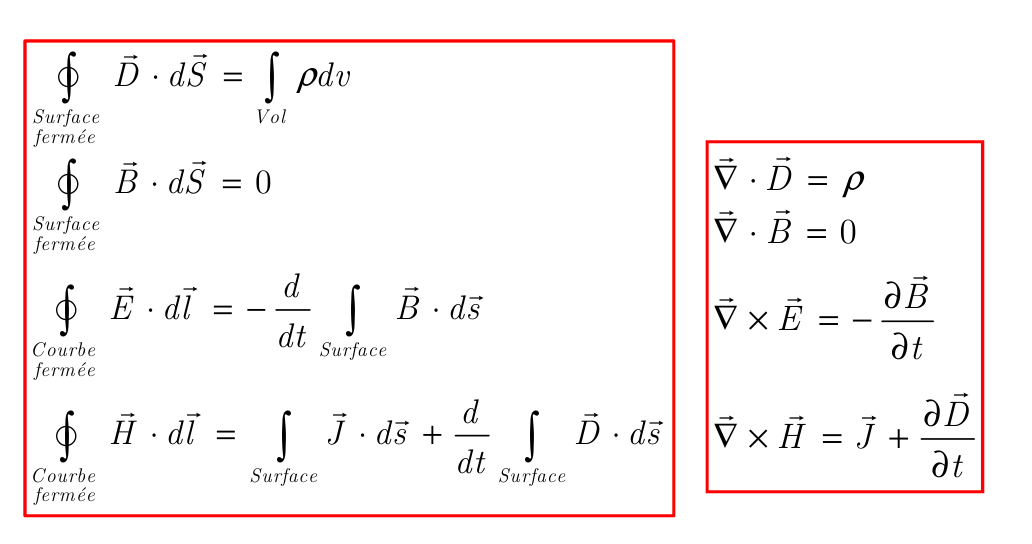
\includegraphics[scale=0.41]{images/maxwell.png} \end{center}
$$\vec{D} = \epsilon \vec{E}$$
$$\vec{B} = \mu \vec{H}$$

Les équations 3 et 4 sont des équations couplées

\subsubsection{Conservation de la charge}

\begin{align*}
\nabla \times \vec{H} &= \vec{J} + \frac{\partial \vec{D}}{\partial t} \\
\nabla \cdot (\nabla \times \vec{H}) &= \nabla \cdot \vec{J} + \frac{\partial}{\partial t} \nabla \cdot \vec{D} = 0 \\
\nabla \cdot \vec{J} + \frac{\partial \rho}{\partial t} &= 0 \qquad \Rightarrow \qquad \boxed{\nabla \cdot \vec{J} = - \frac{\partial \rho}{\partial t}}
\end{align*}

S'il existe un \textbf{flux de courant} non-nul à travers une surface fermée, alors il y a \textbf{accumulation de charges} à l'intérieur de cette surface

$$\boxed{\oint\limits_{S.\text{fermée}} \vec{J} \cdot d\vec{S} = - \frac{\partial}{\partial t} \int\limits_{Vol} \rho \: dv}$$

\subsubsection{Formulation fréquentielle}

Champs sinusoïdaux :

$$\vec{E}(\vec{r}, t) = \mathcal{R}[\vec{\textbf{E}}(\vec{r}) e^{j\omega t}]$$

$\vec{\textbf{E}}(\vec{r})$ est le phaseur complexe représentant le champ sinusoidal

\medskip

Dans le domaine phasoriel (fréquentiel) :
$$\frac{\partial}{\partial t} \rightarrow j\omega$$

\begin{center} 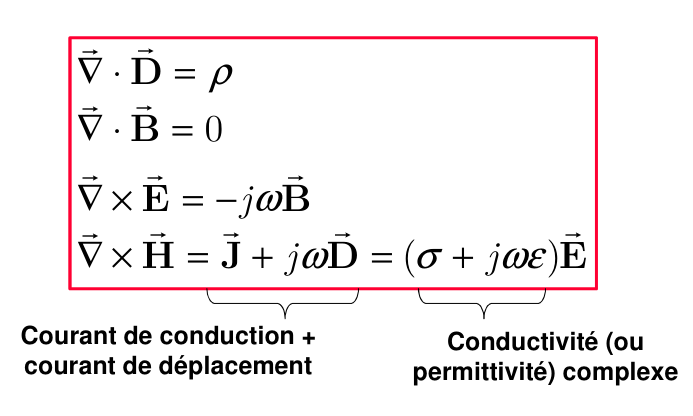
\includegraphics[scale=0.4]{images/maxwell-freq.png} \end{center}

Angle de pertes diélectriques :

$$\tan{\delta} = \frac{\sigma}{\omega \epsilon}$$

Conservation de la charge :
$$\vec{\nabla}\cdot \vec{J} = -j\omega \rho$$


\subsection{Conditions aux interfaces}

\begin{itemize}
        \item Densité surfacique de charge $\rho_s$ : scalaire, en $[\unit{\coulomb\per\meter\squared}]$
        \item Densité de courant de surface $\vec{K}$ : vecteur, en $[\unit{\ampere\per\meter}]$ (par mètre de large)
\end{itemize}

$$\boxed{\vec{n} \cdot (\vec{D}_1 - \vec{D}_2) = \rho_s}$$
$$\boxed{\vec{n} \cdot (\vec{B}_1 - \vec{B}_2) = 0}$$
$$\boxed{\vec{n} \times (\vec{E}_1 - \vec{E}_2) = \vec{0}}$$
$$\boxed{\vec{n} \times (\vec{H}_1 - \vec{H}_2) = \vec{K}}$$

\textbf{Sens du vecteur normal : de $2$ vers $1$}

En appliquant le condition aux interfaces sur le champ $H$ le long d'un contour tangentiel à l'interface, on obtient (après une démonstration) :

$$\boxed{\vec{n} \cdot (\vec{J}_1 - \vec{J}_2) + \text{div}_s \vec{K} + \frac{\partial \rho_s}{\partial t} = 0}$$

($\text{div}_s \vec{K}$ sera toujours égale à $0$ dans les problèmes)

S'il existe un différentiel de courant non-nul entre les 2 côtés d'une interface, alors il y a accumulation de charges à l'interface



\subsection{Potentiels scalaire et vecteur}


\subsubsection{Potentiel électrostatique}

En l'absence de champ $B$ variable (en statique), $E$ est conservatif et dérive d'un potentiel scalaire
$$\boxed{\Delta \phi = -\int_A^B \vec{E} \cdot d\vec{l} = \phi_B - \phi_A} \quad \Leftrightarrow \quad \vec{E} = -\text{grad } \phi \equiv -\nabla \phi$$

Le potentiel est continu aux interfaces

\medskip

On intègre le champ électrique $r$ jusqu'à l'infini pour trouver

$$\phi = \frac{q}{4\pi \epsilon_0 r} = \frac{1}{4\pi\epsilon_0} \int_{V'} \frac{\rho(\vec{r}') dv'}{|\vec{r} - \vec{r}'|}$$


\medskip

Équation de Laplace/Poisson :

$$
\left.
\begin{array}{l}
\vec{E} = -\nabla\phi \\
\vec{\nabla} \cdot \vec{D} = \rho
\end{array}
\right\}
\Rightarrow \vec{\nabla} \cdot \vec{E} = \frac{\rho}{\varepsilon}
\Rightarrow \vec{\nabla} \cdot (-\nabla\phi) = \frac{\rho}{\varepsilon}
\Rightarrow \boxed{\nabla^2\phi = -\frac{\rho}{\varepsilon}}
$$

Si le champ $E$ est non-conservatif :

$$\oint_{\text{Cfermé!}} \vec{E} \cdot \vec{dl} \neq 0$$

$\Rightarrow$ Ce champ ne dérive pas d'un potentiel, n'est pas créé par des charges stationnaires, et son intégrale sur un contour fermé est une fem

\subsubsection{Force électromotrice induite}

Anneau ouvert :

\begin{itemize}
        \item Apparition d'un champ électromoteur (dans l'anneau et dans l'entrefer)
        \item Aucun courant ne circule dans l'anneau $\rightarrow$ le champ $E$ dans l'anneau doit être nul
        \item Apparition d'un champ électrostatique dans l'anneau qui compense le champ électromoteur (conditions limites aux interfaces de l'entrefer sont bien respectées)
\end{itemize}

Anneau fermé :

\begin{itemize}
        \item Apparition d'un champ électromoteur
        \item Induction d'un courant (qui circule dans le même sens que $E_\text{mot}$)
\end{itemize}


\subsubsection{Potentiel-vecteur}

En présence d'un champ magnétique variable, $E$ ne peut pas uniquement dériver d'un potentiel électrostatique

$$\boxed{\vec{E} = -\nabla \phi - \frac{\partial \vec{A}}{\partial t}}$$

$\vec{A}$ est défini tel que $\nabla\times \vec{A} = \vec{B}$ et est appelé \textbf{potentiel-vecteur}

On peut trouver :

$$\vec{A} = \frac{\mu_0}{4\pi} \int_{V'} \frac{\vec{J}(\vec{r'})}{|\vec{r} - \vec{r'}|} \, dv'$$


\subsection{Énergie}

\subsubsection{Rappels}

\begin{itemize}
        \item Énergie dans une capacité : $U_E = \frac{CV^2}{2}$
        \item Densité (volumique) d'énergie électrique ($\epsilon_r$ constant) : $E_E = \frac{\epsilon E^2}{2}$
        \item Énergie dans une inductance : $U_M = \frac{LI^2}{2}$
        \item Densité (volumique) d'énergie magnétique ($\mu_r$ constant) : $E_M = \frac{B^2}{2\mu}$
        
        $E_M = \int_0^{B_\text{max}} H\cdot dB$ si $\mu_r$ non constant (hystérésis)
        \item Puissance dissipée par une résistance : $P_J = RI^2$
        \item Densité (volumique) de puissance dissipée par un courant : $W_J = \sigma E^2$
\end{itemize}

\subsubsection{Théorème de Poynting}

En partant des deux dernières équations de Maxwell, on peut arriver à :

$$\boxed{ \oint_S \vec{E} \times \vec{H} \cdot d\vec{S} = -\int_V \left( \vec{H} \cdot \frac{\partial \vec{B}}{\partial t} + \vec{E} \cdot \frac{\partial \vec{D}}{\partial t} \right) dV - \int_V \vec{E} \cdot \vec{J} dV }$$

En faisant un bilan énergétique, on arrive à

$$\boxed{ -\oint_S \vec{E} \times \vec{H} \cdot d\vec{S} = \frac{\partial}{\partial t} \int_V (E_M + E_E) dV + P_J }$$

Le vecteur de Poynting est $\vec{S} = \vec{E} \times \vec{H}$. Le flux du vecteur de Poynting entrant dans le volume est égal à la variation d'énergie électromagnétique (inductive/capacitive) et la puissance dissipée par effet Joule (résistive)


\subsection{Méthodologie de résolution}

\begin{itemize}
        \item Déterminer la direction des champs
        \subitem Sur base des lois de Coulomb/Gauss ou Biot-Savart/Ampère
        \subitem Sur base des symétries existantes
        \item Déterminer la dépendance (spatiale) des champs
        \subitem Sur base de la géométrie
        \subitem Sur base des symétries
        \item Écrire les équations locales simplifiées
        \item Écrire les conditions de continuité aux interfaces
        \item Résoudre
\end{itemize}

\break
\section{Éléments de circuits localisés}

\subsection{Équivalent EM des lemmes de Kirchhoff}

\begin{center} 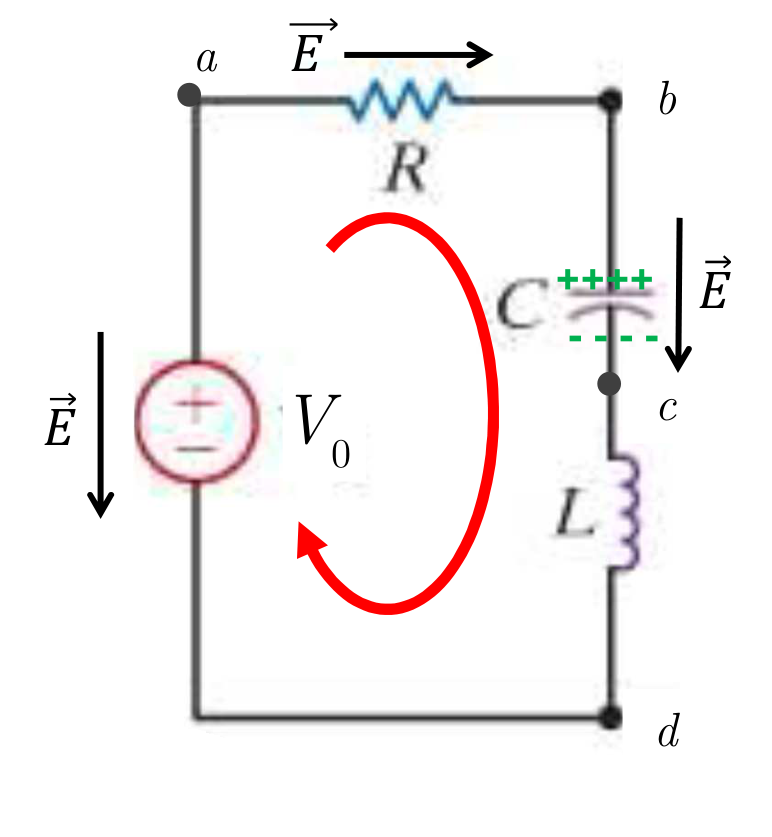
\includegraphics[scale=0.2]{images/equiv-em-kirchhoff.png} \end{center}

$$\oint \vec{E}\cdot d\vec{l} = -\frac{\partial \Phi_B}{\partial t}$$

\begin{align*}
\Rightarrow \int_a^b \vec{E} \cdot d\vec{l} + \int_b^c \vec{E} \cdot d\vec{l} + \int_c^d \vec{E} \cdot d\vec{l} + \int_d^a \vec{E} \cdot d\vec{l} &= -\oint \frac{\partial \vec{B}}{\partial t} \cdot d\vec{S} \\
\int_a^b \frac{\vec{J}_R}{\sigma} \cdot d\vec{l} + \int_b^c \nabla\phi_C \cdot d\vec{l} + \underbrace{\int_c^d \vec{E} \cdot d\vec{l}}_{=0} - V_0 &= \underbrace{-\oint \frac{\partial \vec{A}}{\partial t} \cdot d\vec{l}}_{\text{Stokes}, \nabla \times \vec{A} = \vec{B}} \\
\Rightarrow \int_a^b \frac{\vec{J}_R}{\sigma} \cdot d\vec{l} + \int_b^c \nabla\phi_C \cdot d\vec{l} + \oint \frac{\partial \vec{A}}{\partial t} \cdot d\vec{l} &= V_0 \Leftrightarrow \underbrace{RI + \frac{1}{C}\int I dt + L \frac{dI}{dt} = V_0}_\text{Loi des mailles}
\end{align*}

\textbf{Autre formulation} :

\begin{itemize}
        \item Champ lié aux charges/courants : $\vec{E} = -\nabla \phi - \frac{\nabla \vec{A}}{\partial t}$
        \item Champ (électromoteur) de source : $\vec{E}_0$
        
        (n'existe que dans la source, $V_0 = \int_d^a \vec{E}_0\cdot d\vec{l}$)
        \item Champ total : $\vec{E}_t = \vec{E}_0 + \vec{E} = \frac{\vec{J}}{\sigma} \Rightarrow \vec{E}_0 = \frac{\vec{J}}{\sigma} - \vec{E}$
\end{itemize}
$$\Rightarrow \vec{E}_0 = \frac{\vec{J}}{\sigma} + \nabla \phi + \frac{\partial \vec{A}}{\partial t} \Leftrightarrow V_0 = RI + \frac{1}{C}\int I dt + L \frac{dI}{dt} $$

\textbf{Conservation de la charge (pas de courant de surface)} :

$$
\vec{n} \cdot (\vec{J}_1 - \vec{J}_2) + \frac{\partial \rho_S}{\partial t} = 0 \Rightarrow -\vec{J}_R + \frac{\partial \rho_S}{\partial t} = 0
$$
$$
\Rightarrow \vec{J}_R = \frac{\partial \rho_S}{\partial t} = \frac{\partial(\vec{n} \cdot \vec{D})}{\partial t} \Leftrightarrow \underbrace{I = C \frac{dV_C}{dt}}_\text{Loi des noeuds aux points b (et c)}
$$


\subsection{Résistance}

$$\boxed{\vec{J} = \sigma \vec{E}}$$

La conductivité $\sigma$
\begin{itemize}
        \item est indépendante du champ et du courant
        \item dépend de la température
        \item est isotrope dans les métaux
\end{itemize}

$$R = \frac{L}{\sigma S}$$

De manière générale :

$$\boxed{ R = \frac{\int_a^b \vec{E} \cdot d\vec{l}}{\int_S \vec{J} \cdot d\vec{S}} = \frac{-\int_b^a \vec{E} \cdot d\vec{l}}{\int_S \sigma \vec{E} \cdot d\vec{S}} = \frac{\Delta V_R}{I} }$$

\subsubsection{En régime alternatif}

Dans un bon conducteur en courant alternatif, les champs EM sont rejetés à la surface. Ils ne pénètrent pas au-delà de quelques "profondeurs de peau"

$$\delta = \sqrt{\frac{2}{\omega \mu \sigma}}$$

$\delta$ est la profondeur à laquelle le champ a diminué de $e^{-1}$


\subsection{Capacité}

$$\boxed{C = \frac{Q}{V_0}}$$

La capacité exprime le rapport entre la charge et la différence de potentiel

$$\boxed{
C = - \frac{Q}{\displaystyle\int_c^b \nabla \phi_C \cdot d\vec{l}}
= - \frac{\displaystyle\int_S \vec{D} \cdot d\vec{S}}{\displaystyle - \int_c^b \vec{E} \cdot d\vec{l}}
= \frac{\displaystyle\int_S \varepsilon \vec{E} \cdot d\vec{S}}{\displaystyle\int_c^b \vec{E} \cdot d\vec{l}}
}$$


\subsection{Inductance}

$$\boxed{L = \frac{\int_S \vec{B} \cdot d\vec{S}}{I} = \frac{\Phi}{I} = \frac{\int_S \vec{B} \cdot d\vec{S}}{\oint \vec{H} \cdot d\vec{l}}}$$

L'inductance exprime le rapport entre le flux magnétique et le courant qui a créé ce flux

\begin{comment}
\subsubsection{Inductance mutuelle}

\begin{center} 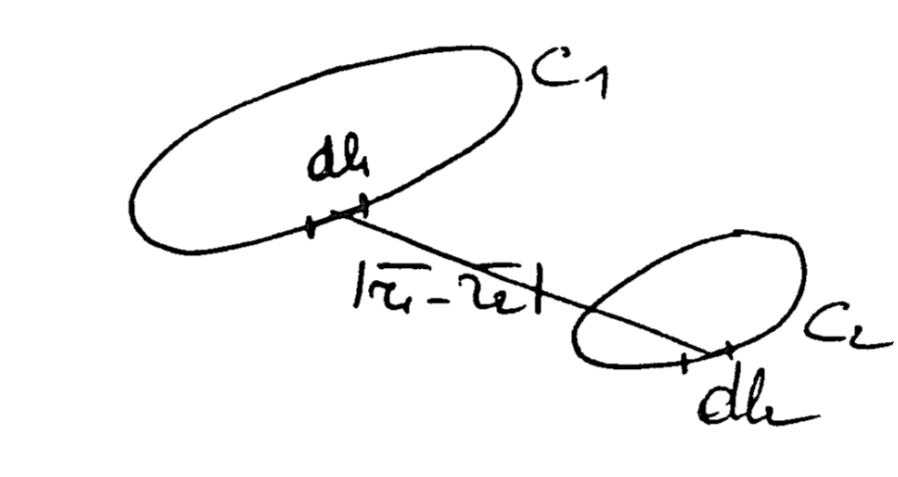
\includegraphics[scale=0.2]{images/inductance-mutuelle.png} \end{center}
$$L_{12} = L_{21} = \frac{\mu}{4\pi} \int_{C_1} \int_{C_2} \frac{d\vec{l}_1 \cdot d\vec{l}_2}{|\vec{r}_1 - \vec{r}_2|}$$
\end{comment}

\break

\section{Circuits distribués}

\subsection{Limite de la représentation par éléments localisés}

On prend deux cas, le premier deux plaques parallèle avec une plaque (de résistance $R_c$) qui les relie, et le deuxième sans la plaque qui relie les deux plaques parallèles

\begin{center} 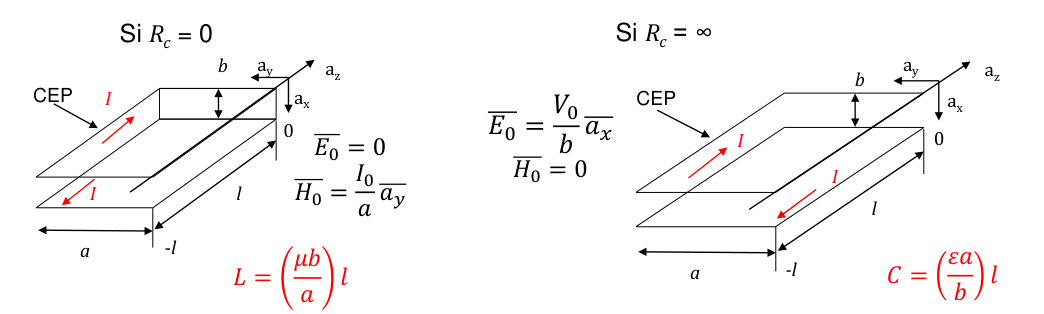
\includegraphics[scale=0.4]{images/limite-local.png} \end{center}

On décompose en série des champs en fonction de la fréquence
$$E_x = E_{x0} + E_{x1}\omega + E_{x2}\omega^2 + \dots$$
$$H_y = H_{y0} + H_{y1}\omega + H_{y2}\omega^2 + \dots$$
$$E_{xn},H_{yn} = f(z,\text{géométrie})$$

Après un long calcul, on obtient

$$V = I_0R_c [\cosh(j\beta_0 z) - \chi \sinh(j\beta_0 z)]$$
$$I = aH_y = I_0\left[\cosh(j\beta_0z) - \frac{1}{\chi}\sinh(j\beta_0 z)\right]$$

Avec

$$\beta_0 = \omega \sqrt{\epsilon\mu} \quad ; \quad \eta = \sqrt{\frac{\mu}{\epsilon}} \quad ; \quad \chi = \frac{\eta}{r} \quad ; \quad R_c = b\frac{r}{a}$$

Ce sont des solutions de l'équation d'ondes ($e^{\pm j\beta z}$)

La structure n'est ni une capacité, ni une inductance, mais le siège d'une \textbf{onde de tension} $V(z,t) = f_V(\omega t \pm \beta z) \neq V(t)$ et d'une \textbf{onde de courant} $I(z,t) = f_I(\omega t \pm \beta z) \neq I(t)$

Les différents termes de la décomposition en série sont de la forme $(j\beta_0 l)^n$ et dépendent donc du rapport $l/\lambda$ entre la longueur de l'élément et la longueur d'onde


\subsection{Champs dans les lignes de transmission}

Les lignes usuelles sont \textbf{uniformes}, leur configuration transverse est indépendante de $z$.

Une ligne de transmission est capable de guider un grand nombre de \textbf{modes}, mais en général on prend des fréquences telles qu'un seul mode se propage

Dans ce cours on s'intéresse aux ondes planes.

\textbf{Plan transverse} : Plan perpendiculaire à la direction de propagation ($z$)

\begin{itemize}
        \item \textbf{Onde TEM} : Les champs électrique et magnétique sont entièrement transverses
        \item \textbf{Onde TE} : Seul le champ électrique est purement transverse, le champ magnétique a une composante longitudinale
        \item \textbf{Onde TM} : Seul le champ magnétique est purement transverse, le champ électrique a une composante longitudinale
\end{itemize}

\subsubsection{Ondes TEM}

\textbf{Propriété des ondes TEM} : Leur composantes obéissent aux équations de la statique dans le plan transverse

$\rightarrow$ Dans le plan transverse (en tout $z$ donné), représentation par un circuit localisé (valable uniquement pour longueur $dz$ infinitésimale)

\medskip

\textbf{Gradient spatial dans le plan transverse} :
$$\nabla = \nabla_t + \bar{a_z}\frac{\partial}{\partial z}$$
avec $\nabla_t = \bar{a_x} \frac{\nabla}{\nabla x} + \bar{a_y}\frac{\partial}{\partial y}$

$\bar{a_z}$ est le vecteur unitaire dans la direction $z$

\bigskip

En appliquant cette décomposition aux équations de Maxwell, on trouve sur le plan $z$ :

$$\left\{ \begin{array}{l} \nabla_t \times \bar{E}_t = 0 \\ \nabla_t \times \bar{H}_t = 0 \end{array} \right.$$
\begin{align*}
\bar{a}_z \times \frac{\partial \bar{E}_t}{\partial z} &= -\mu \frac{\partial \bar{H}_t}{\partial t} \\
\bar{a}_z \times \frac{\partial \bar{H}_t}{\partial z} &= \varepsilon \frac{\partial \bar{E}_t}{\partial t} + \sigma \bar{E}_t
\end{align*}
$$\bar{E}_t \perp \bar{H}_t$$

\medskip

Dans un CEP (conducteur électrique parfait), on ne peut avoir ni champ électrique, ni champ magnétique variable dans le emps

$\rightarrow$ Mêmes conditions aux limites qu'en statique

$\rightarrow$ Pas d'onde TEM à l'intérieur d'un tube creux en CEP ($\bar{E}=\bar{0}$)

$\rightarrow$ Pour une onde TEM, il faut au monis $2$ conducteurs

Dans un milieu sans pertes, le terme $\sigma \bar{E}_t$ est nul

Puisque c'est un milieu sans pertes et sans charges, $\nabla_t \cdot \bar{E_t} = 0$

Le rotationnel du champ électrique transverse est nul, il dépend donc d'un potentiel scalaire :
$$\bar{E_t} \triangleq - \nabla_t \phi \quad \text{ou} \quad \nabla_t^2 \phi = 0$$


\bigskip

On travaille en phaseurs + propagation en $z$

$\rightarrow$ La dépendance en $z$ s'écrit uniquement via $e^{-j\beta z}$

\begin{itemize}
        \item Lorsqu'on dérive par rapport à $t$, en fréquentielle on fait $\times j\omega$
        \item Lorsqu'on dérive par rapport à $z$, en fréquentielle on fait $\times j\beta$
\end{itemize}

On trouve donc
$$\bar{H}_t = \frac{\beta}{\omega \mu} \bar{a}_z \times \bar{E}_t$$

\subsubsection{Équation de Helmoltz}

On peut trouver que
$$\boxed{\beta = \omega\sqrt{\epsilon\mu} = \omega/c = \frac{2\pi}{\lambda}}$$

\medskip

Soit l'admittance du milieu 
$$Y \triangleq \sqrt{\frac{\epsilon}{\mu}} \quad \text{et} \quad Y_0 = \sqrt{\frac{\epsilon_0}{\mu_0}} \; \text{dans le vide}$$
On peut écrire le champ magnétique sous la forme
$$\bar{H}_t = Y\bar{a}_z \times \bar{E}_t = Y\bar{a}_z \times (-\nabla_t \Phi e^{-j\beta z})$$
$$\textbf{car} \quad \frac{\beta}{\omega\mu} = \frac{\omega\sqrt{\varepsilon\mu}}{\omega\mu} = \sqrt{\frac{\varepsilon}{\mu}} = Y$$


\subsubsection{Paramètres fondamentaux}

\begin{itemize}
        \item On définit une \textbf{Onde de tension} :
        $$V(z) = V_0 e^{-j\beta z} \qquad \text{avec} \quad V_0 \triangleq \int_{C_1}^{C_2} \nabla_t \Phi\cdot \overline{dl}$$

        \item On définit une \textbf{Onde de courant} :
        $$I(z) = I_0 e^{-j\beta z} \qquad \text{avec} \quad I_0 \triangleq \oint_C Y\bar{a_z} \times \left(-\nabla_t \Phi\right)\cdot\overline{dl}$$
        car $\bar{H_t} = Y\bar{a_z} \times \bar{E_t} = Y\bar{a_z} \times \left(-\nabla_t \Phi e^{-j\beta z}\right)$
\end{itemize}

\textbf{Impédance caractéristique} :
$$Z_c = \frac{1}{Y_c} \triangleq \frac{V_0}{I_0}$$

\begin{itemize}
        \item $Z_c$ n'est pas l'impédance d'onde
        \item $Z_c$ est le rapport des aplitudes des ondes de tension et de courant \textbf{se déplacant dans un même sens}
\end{itemize}

\textbf{Puissance électromagnétique traversant le plan transverse} :

$$
P = \underbrace{\frac{1}{2} \mathrm{Re} \int_A \bar{E} \times \bar{H}^* \cdot d\bar{a}}_\text{intégrale du vecteur de Poynting sur la section}
  = \frac{1}{2} \mathrm{Re} \int_A \bar{E}_t \times \bar{H}_t^* \cdot \bar{a}_z da
  = \underbrace{\frac{1}{2} \mathrm{Re} (VI^*)}_\text{définition “circuits”}
$$



\subsubsection{Résumé}

\begin{center} 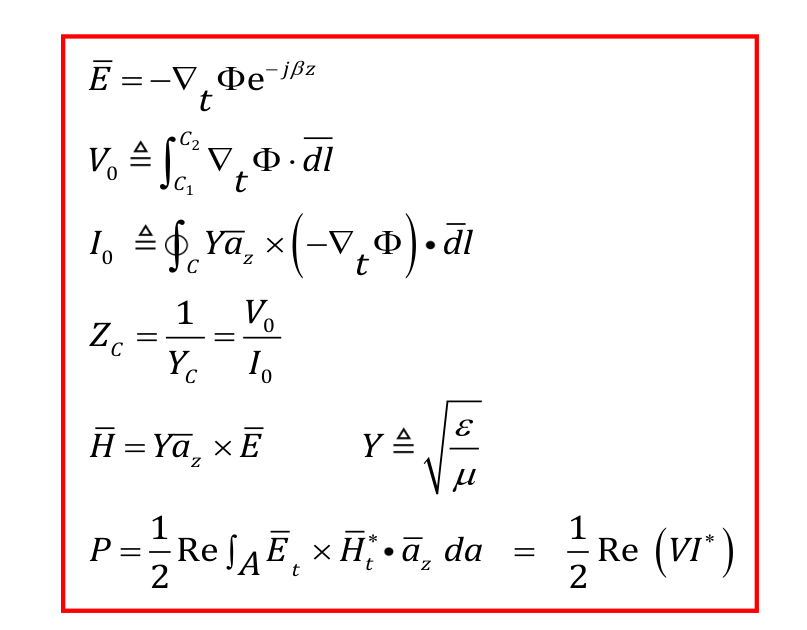
\includegraphics[scale=0.45]{images/resume.png} \end{center}


\subsubsection{Paramètres linéiques}

\begin{itemize}
        \item \textbf{Capacité linéique} :
        
        $$C = \frac{\rho_l}{V_0}$$
        $$Z_c = \frac{V_0}{I_0} = \frac{\rho_l / C}{Y \rho_1 / \epsilon} = \frac{Z\epsilon}{C} \qquad \text{ou} \qquad Z_c = \frac{\sqrt{\epsilon\mu}}{C} = \frac{1}{vC}$$

        \item \textbf{Inductance linéique} :
        
        $$L = \frac{\phi}{I_0}$$
        $$L = \mu Y \frac{V_0}{I_0} = \mu Y Z_c = \frac{Z_c}{v}$$
\end{itemize}

Pour des lignes sans pertes, on obtient :

$$\boxed{Z_c = \sqrt{L/C}} \qquad \boxed{v = 1/\sqrt{LC}} \qquad \boxed{LC = \epsilon \mu} \qquad \boxed{\beta = \omega\sqrt{LC}}$$


\subsection{Lignes de transmission avec pertes}

\begin{itemize}
        \item \textbf{Pertes dans le milieu} : Caractérisé par une permittivité complexe $\epsilon' - j\epsilon''$ ou par combinaison d'une permittivité et d'une conductivité
        \item \textbf{Pertes dans les conducteurs} : Ceux-ci ne sont pas parfaits $\epsilon - j\sigma/\omega$
\end{itemize}

Dans les deux cas, on obtient un exposant de propagation complexe
$$\alpha + j\beta$$
La dépendance en $z$ du phaseur devient
$$e^{-\gamma z} = e^{-\alpha z} e^{-j\beta z}$$

\subsubsection{Pertes dans le milieu}

$$\boxed{\bar{J} = \sigma \bar{E} \quad \text{ou} \quad \bar{J} = \omega \epsilon'' \bar{E}}$$

On introduit une solution du type $e^{-\gamma z}$ dans les équation de Maxwell

En faisant un raisonnement similaire au cas sans pertes, on obtient
$$\gamma = \alpha + j\beta = \sqrt{j\omega\mu (\sigma + j\omega\epsilon)}$$

En résolvant cette équation, on trouve
\begin{align*}
\beta^2 &= \left(\frac{\omega^2 \varepsilon \mu}{2}\right) \left[ \sqrt{1 + \left(\frac{\sigma}{\omega \varepsilon}\right)^2} + 1 \right] \\
\alpha^2 &= \left(\frac{\omega^2 \varepsilon \mu}{2}\right) \left[ \sqrt{1 + \left(\frac{\sigma}{\omega \varepsilon}\right)^2} - 1 \right]
\end{align*}

Rappel : vitesse de phase $v_{ph} = \omega\sqrt{\epsilon\mu}$

Si $\sigma = 0$, on revient au résultat sans pertes

On a toujours
$$\beta \geq \omega\sqrt{\epsilon\mu} \quad \text{et} \quad \alpha \leq \beta$$

\bigskip

\textbf{Dans un bon diélectrique} :

On peut développer en série, en faisant l'hypothèse que $\sigma/\omega\epsilon << 1$, et garder le premier ordre
$$\beta \approx \omega \sqrt{\epsilon\mu}$$
$$\alpha \approx \frac{\omega}{2} \sqrt{\frac{\mu}{\epsilon}}$$

$\beta$ identique au cas sans pertes, et $\alpha$ atténué par $\sigma$

%<Représentation circuits, 17.2>

\textbf{Dans un bon conducteur} :

L'onde ne peut plus vraiment être TEM, mais on fait l'hypothèse qu'elle est quasi-TEM, on obtient en faisant l'hypothèse que $\omega\epsilon / \sigma << 1$
\begin{flalign*}
        \beta &\approx \sqrt{\omega\mu\sigma/2}\\
        \alpha &\approx \sqrt{\omega\mu\sigma/2} = \delta^-1 \qquad \text{$\delta\equiv$ profondeur de peau}\\
        \gamma &\approx \sqrt{j \omega \mu \sigma}
\end{flalign*}

Circuit équivalent d'une ligne TEM :
\begin{itemize}
        \item Onde TEM $\rightarrow$ L,C
        \item Pertes milieu $\rightarrow$ G (généralement faible)
        \item Pertes conducteurs $\rightarrow$ R (généralement faible)
\end{itemize}

\textbf{Circuit équivalent} infinitésimal (circuit distribué) pour une longueur $dz$ :
\begin{center} 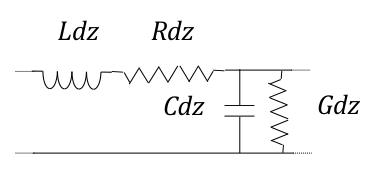
\includegraphics[scale=0.5]{images/circuit-dz.png} \end{center}

\begin{center} 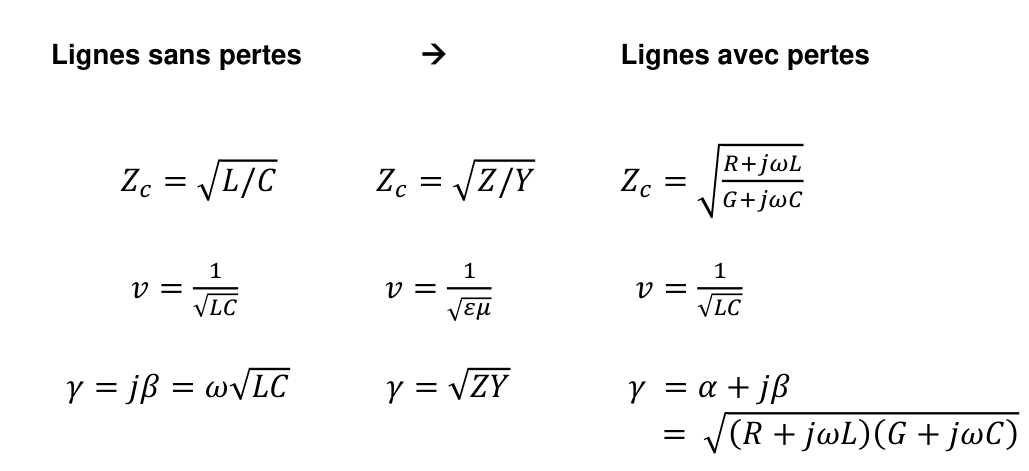
\includegraphics[scale=0.4]{images/ligne-perte.png} \end{center}


\break

\section{Lignes de transmission}

\subsection{Quadripôle équivalent}

\subsubsection{Circuit distribué}

\begin{center} 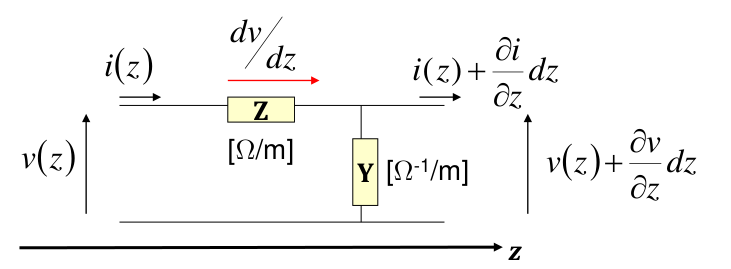
\includegraphics[scale=0.4]{images/ligne-quadri.png} \end{center}

Lignes uniformes (Z, Y constantes) :
$$Z = R + j\omega L \qquad ; \qquad Y = G + j\omega C$$

\begin{comment}
$$\left\{\begin{array}{l}
-\frac{dV(z, p)}{dz}=Z I(z, p) \\
-\frac{dI(z, p)}{dz}=Y V(z, p)
\end{array}\right. \quad \text{On dérive} \rightarrow \quad \left\{\begin{array}{l}
-\frac{d^2V(z, p)}{dz^2}=Z \frac{dI(z, p)}{dz} \\
-\frac{d^2I(z, p)}{dz^2}=Y \frac{dV(z, p)}{dz}
\end{array}\right.$$
\end{comment}

En résolvant le circuit, on peut trouver l'équation des télégraphistes :

$$\boxed{\begin{cases}
\frac{d^2 V}{d z^2} = ZYV \\
\frac{d^2 I}{d z^2} = ZYI
\end{cases}}$$

\subsubsection{Ondes de tension et de courant}

En résolvant l'équantion des télégraphistes, on trouve
\begin{align*}
V(z) &= V_{+} e^{-\sqrt{ZY} z} + V_{-} e^{\sqrt{ZY} z} \\
I(z) &= I_{+} e^{-\sqrt{ZY} z} + I_{-} e^{\sqrt{ZY} z}
\end{align*}

avec
$$I_+ = \sqrt{\frac{Y}{Z}} \, V_+ \qquad ; \qquad
I_- = -\sqrt{\frac{Y}{Z}} \, V_-
$$

Impédance caractéristique et exposant de propagation :
$$
\boxed{Z_c \triangleq \sqrt{\frac{Z}{Y}} = R_c + jX_c} \qquad ; \qquad
\boxed{\gamma \triangleq \sqrt{ZY} = \alpha + j\beta}
$$

On a donc
\label{eq-onde}
$$\boxed{\begin{cases}
V(z) = V_+ e^{-\gamma z} + V_- e^{\gamma z} \\
I(z) = Y_c \left[ V_+ e^{-\gamma z} - V_- e^{\gamma z} \right]
\end{cases}}$$


\subsubsection{Ligne de longueur donnée}

\begin{center} 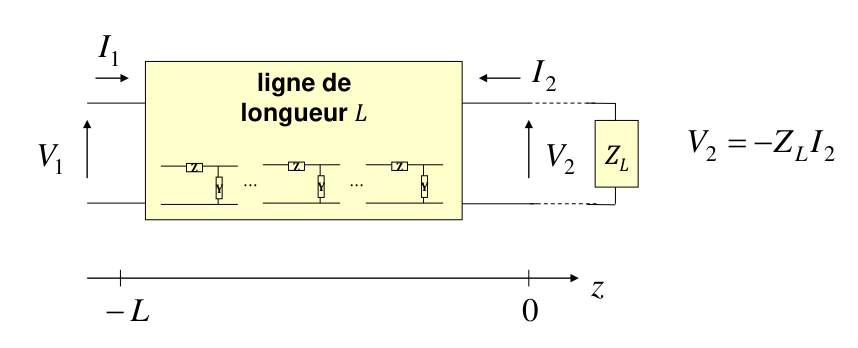
\includegraphics[scale=0.4]{images/ligne-l.png} \end{center}
$$V_1 = V(-L) \qquad ; \qquad V_2 = V(0) \qquad I_1 = I(-L) \qquad ; \qquad I_2 = -I(0)$$

On peut trouver :
$$\boxed{\begin{bmatrix} V_1\\ I_1\end{bmatrix} = \begin{bmatrix}
\cosh(\gamma L) & Z_c \sinh(\gamma L) \\
Y_c \sinh{\gamma L} & \cosh(\gamma L)
\end{bmatrix} \begin{bmatrix}
        V_2 \\ - I_2
\end{bmatrix}} = \begin{bmatrix}
A & B \\
C & D
\end{bmatrix} \begin{bmatrix}
V_2 \\ - I_2
\end{bmatrix} $$



\subsubsection{Impédance d'entrée d'une ligne chargée}

$$Z_{in} = \frac{V_1}{I_1}\Bigg|_{Z_L} = \frac{B + A Z_L}{D + C Z_L} = \boxed{Z_c \frac{Z_c + Z_L \coth (\gamma L)}{Z_L + Z_c \coth (\gamma L)}}$$
\begin{itemize}
        \item Ligne ouverte : $\;\;\;\qquad\quad Z_L = \infty \rightarrow Z_{in} = Z_c \coth (\gamma L)$
        \item Ligne court-circuitée : $\quad Z_L = 0 \rightarrow Z_{in} = Z_c \tanh (\gamma L)$
        \item Ligne "adaptée" : $\quad\qquad Z_L = Z_c \rightarrow Z_{in} = Z_c$
\end{itemize}

\subsubsection{Impédance le long de la ligne}

$$Z(z) = \frac{V(z)}{I(z)} = -\frac{V_2 \cosh(\gamma z) + Z_c I_2 \sinh(\gamma z)}{Y_c V_2 \sinh(\gamma z) + I_2 \cosh(\gamma z)}$$

Si $V_2 = Z_L I_2$ (ligne chargé par une impédance $Z_L$) :
$$ Z(z) = Z_c \frac{Z_c - Z_L \coth(\gamma z)}{Z_L - Z_c \coth(\gamma z)} $$



\subsection{Réflexion et taux d'ondes stationnaires}

\subsubsection{Onde progressive}

La solution générale des équations (voir \ref{eq-onde}) est constituée de deux ondes progressives, l'une vers les $z>0$ et l'autre vers les $z<0$.

Pour une ligne de longueur infinie, ou pour une ligne adaptée, $V_- = 0$
$$\begin{cases}
V(z) = V_+ e^{-\gamma z} \\
Z_c I(z) = V_+ e^{-\gamma z}
\end{cases}
\Rightarrow
Z(z) = Z_c
$$

On a une onde progressive pure

\subsubsection{Cas général}

$$V(z) = \underbrace{V_+ e^{-\gamma z}}_\text{incidente} + \underbrace{V_- e^{\gamma z}}_\text{réfléchie}$$

\begin{enumerate}
        \item \textbf{Ligne ouverte à son extrémité} $\Rightarrow I_2 = 0 = V_+-V_-$

        $v(z,t) = 2V_+ \cos(\omega t)\cos(\beta z) \qquad \rightarrow \quad \text{Apparition d'une onde purement stationnaire}$
        
        $i(z,t) = 2Y_c V_+ \sin(\omega t) \sin(\beta z)$

        \item \textbf{Ligne court-circuitée à son extrémité} $\Rightarrow V_2 = 0 = V_++V_-$

        $v(z,t) = 2V_+ \sin(\omega t)\sin(\beta z) \qquad \rightarrow \quad \text{Apparition d'une onde purement stationnaire}$
        
        $i(z,t) = 2Y_c V_+ \cos(\omega t) \cos(\beta z)$

        \item \textbf{Ligne chargée à son extrémité} $\Rightarrow V_2 = -Z_L I_2$

        On définit un facteur de réflexion en tout $z$ :
        $$\boxed{\Gamma(z) \triangleq \frac{V_- e^{\gamma z}}{V_+ e^{-\gamma z}} = \frac{V_-}{V_+} e^{2\gamma z}}$$

        $$\Rightarrow\begin{cases}
        V(z) = V_+ e^{-\gamma z} \left[ 1 + \Gamma(z) \right] \\
        I(z) = Y_c V_+ e^{-\gamma z} \left[ 1 - \Gamma(z) \right]
        \end{cases}
        \quad \Rightarrow \quad
        Z(z) = Z_c \frac{1 + \Gamma(z)}{1 - \Gamma(z)} = \frac{V(z)}{I(z)}$$

        Lien avec la charge $Z_L$ en $z=0$
        $$\Gamma(0) = \Gamma_L = \frac{V_-}{V_+} \qquad \text{or} \quad V(0) = V_2 = V_+ + V_- \quad \text{et} \quad I(0) = I_2 = Y_c(V_+ - V_-)$$
        $$\Rightarrow \Gamma_L = \frac{Z_L - Z_c}{Z_L + Z_c} \Rightarrow \boxed{\Gamma(z) = \frac{V_-}{V_+} e^{2\gamma z} = \Gamma_L e^{2\gamma z} = \frac{Z_L - Z_c}{Z_L + Z_c} e^{2\gamma z}}$$
        La ligne est le siège d'une onde dont l'\textbf{enveloppe est stationnaire} :
        \begin{align*}
        |V(z)| &= e^{-\alpha z} |V_+| |1 + \Gamma(z)|  \\
        |I(z)| &= e^{-\alpha z} |Y_C| |V_+| |1 - \Gamma(z)|
        \end{align*}
        $\rightarrow$ L'amplitude de la tension est \textbf{maximale} aux positions $z$ telles que $\Gamma(z)$ est \textbf{réel positif}
        
        $\rightarrow$ L'amplitude de la tension est \textbf{minimale} aux positions $z$ telles que $\Gamma(z)$ est \textbf{réel négatif}
\end{enumerate}

\subsubsection{Facteur de réflexion}

Le facteur $\Gamma(z)$ est le paramètre qui permet de tout retrouver

$$|\Gamma(z_1)| = |\Gamma(z_2)| e^{2\alpha(z_1 - z_2)}$$
$$\arg \Gamma(z_1) = \arg \Gamma(z_2) + 2\beta(z_1 - z_2)$$

\begin{center} 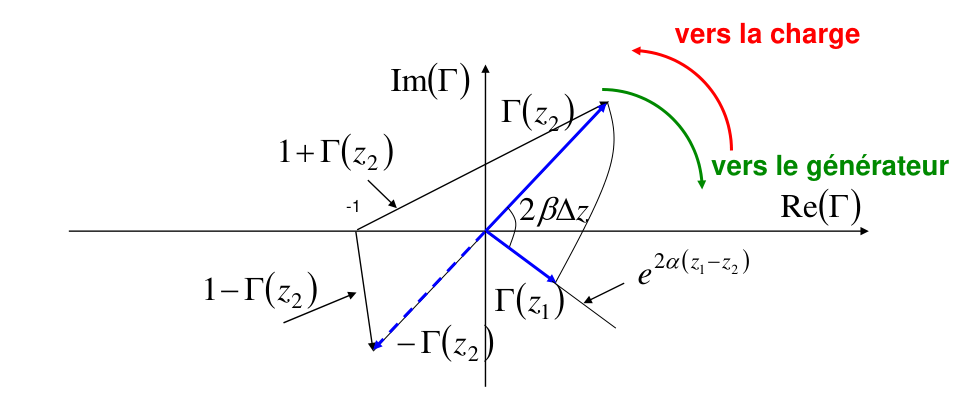
\includegraphics[scale=0.4]{images/fact-reflex.png} \end{center}

$2\beta \Delta z = 2\pi \quad \rightarrow \quad \Delta z = \frac{\pi}{\beta} = \frac{\lambda}{2}$

\subsubsection{Taux d'ondes stationnaires}

En l'absence de pertes, l'amplitude de $\Gamma(z)$ est constante
$$|V(z)| = |V_+||1 + \Gamma(z)| \qquad ; \qquad |I(z)| = |I_+||1-\Gamma(z)|$$
$$\Rightarrow \quad |V(z)|_\text{max} = |V_+| (1 + |\Gamma(z)|) \qquad ; \qquad |V(z)|_\text{min} = |V_+|(1 - |\Gamma(z)|)$$

$$\boxed{\text{TOS ou VSWR} \triangleq \frac{|V(z)|_\text{max}}{|V(z)|_\text{min}} = \frac{1 + |\Gamma(z)|}{1 - |\Gamma(z)|} = s}$$

$$|\Gamma(z)| = \frac{s-1}{s+1}$$



\subsection{Adaptation au sens des lignes de transimission}

\subsubsection{Puissance}

\begin{align*}
P &= \frac{1}{2} V I^* \\
&= \frac{1}{2} V_+ e^{-\gamma z} [1 + \Gamma(z)] Y_c^* V_+^* e^{-\gamma^* z} [1 - \Gamma^*(z)] \\
&= \frac{1}{2} |V_+|^2 Y_c^* e^{-2\alpha z} \left(1 - |\Gamma|^2 + 2j \operatorname{Im} \Gamma\right)
\end{align*}

\begin{equation*}
\operatorname{Re}(P) = \frac{1}{2} |V_+|^2 \operatorname{Re} Y_c \, e^{-2\alpha z} \left( 1 - |\Gamma|^2 + 2 \operatorname{Im} \Gamma \frac{\operatorname{Im} Y_c}{\operatorname{Re} Y_c} \right)
\end{equation*}


\subsubsection{Lignes sans pertes}

Pour une ligne \textbf{sans pertes} ($\gamma=j\beta$ et $Z_c = R_c$), on peut écrire

\begin{align*}
V(z) &= V_+ e^{-j\beta z} + V_- e^{j\beta z} \\
R_c I(z) &= V_+ e^{-j\beta z} - V_- e^{j\beta z}
\end{align*}

$$\boxed{Z(z) = R_c \frac{Z_L - jR_c \tan \beta z}{R_c - jZ_L \tan \beta z} = R_c \frac{Z_L\cos(\beta z) - jR_c\sin(\beta z)}{R_c\cos(\beta z) + j Z_L \sin(\beta z)}}$$

\begin{align*}
\Gamma(z) &= \frac{V_{-}}{V_{+}} e^{2j\beta z} = \Gamma_{L} e^{2j\beta z} \\
\Gamma_{L} &= \frac{Z_{L} / Z_{c} - 1}{Z_{L} / Z_{c} + 1} = \frac{Z_{L} - Z_{c}}{Z_{L} + Z_{c}}
\end{align*}

$$\Gamma(z) = \frac{Z(z) - R_c}{Z(z) + R_c}$$


$$R_e(P) = \frac{1}{2} |V_+|^2 \underbrace{(1 - |\Gamma|^2)}_{>0}/R_c$$

$$\Rightarrow |\Gamma_L| \leq 1 \quad \text{en tout point de la ligne}$$

si $\Gamma = 0$, toute la puissance incidente est transmise

Adapter au sens des lignes de transmission, c'est annuler le coefficient de réflexion au générateur et obtenir $Z_{IN}=R_S$

\subsubsection{Abaque de Smith}

\begin{comment}
On décompose $\frac{Z(z)}{R_c} = R + jX$, et $\Gamma(z) = a + jb$

\begin{center} 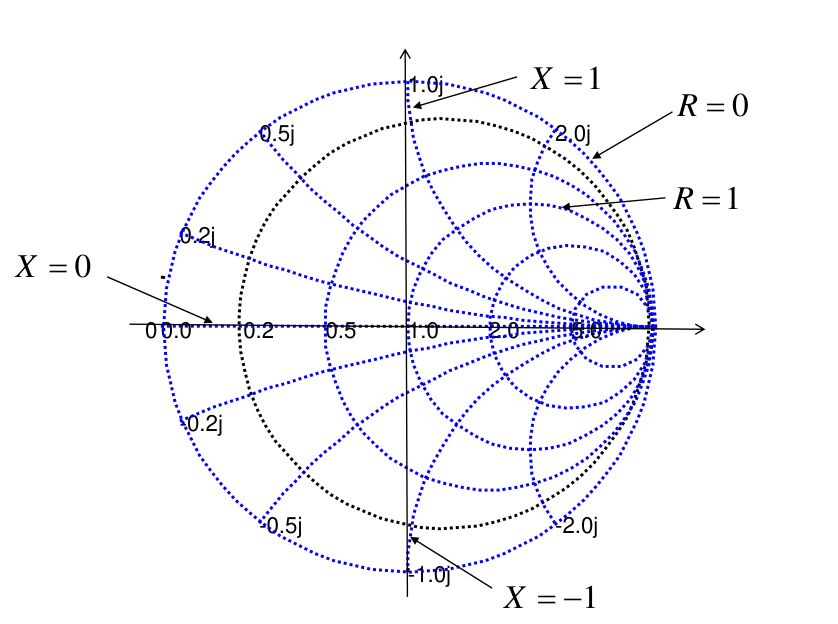
\includegraphics[scale=0.4]{images/smith.png} \end{center}

\begin{itemize}
        \item Chaque cercle correspond à une valeur de $R$
        \item Chaque courbe correspond à une valeur de $X$
        \item $\Gamma$ est le point correspondant sur le plan complexe
\end{itemize}
\end{comment}

Méthode graphique pour calculer l'impédance $Z_{in}$ en utilisant l'abaque de Smith :
\begin{itemize}
        \item Calculer l'impédance de charge normalisée $z_L = \frac{Z_L}{Z_C}$
        \item Calculer l'impédance d'entrée normalisée $z_{in}$ :
        \begin{itemize}
                \item Placer l'impédance de charge normalisée $z_L$ dans l'abaque selon ses parties réelle et imaginaire
                \item Faire une rotation de ce point autour du centre de l'abaque, dans le sens horloger (on va vers le générateur), de $\theta = 4\pi \frac{l}{\lambda}$
        \end{itemize}
        \item Calculer l'impédance d'entrée $Z_{in} = z_{in} Z_C$
\end{itemize}

Astuce : Dans ce cours quand on doit trouver un $Z_C$ ou $Y_C$, il sera uniquement réel







\end{document}
